\documentclass[11pt]{article}
\usepackage{mathtools}
\usepackage{mdframed}
\usepackage{fullpage}
\usepackage{amsfonts}
\usepackage{tikz}
\usepackage{fancyhdr}
\usepackage{lastpage}
\usetikzlibrary{automata, positioning}


%edit this for each class
\newcommand\name{John Collin Vincent}
\newcommand\classname{Com S 311}
\newcommand\assignment{Homework 6}


\newcounter{excounter}
\setcounter{excounter}{1}
\newcommand\ques[2]{\vskip 1em  \noindent\textbf{\arabic{excounter}\addtocounter{excounter}{1}.} \emph{#1} \noindent#2}
\newenvironment{question}{\ques{}\begin{quote}}{\end{quote}}
\newenvironment{subquestion}[1]{#1) \begin{quote}}{\end{quote}}

\pagestyle{fancy}
\rfoot{\name, page \thepage/\pageref{LastPage}}
\cfoot{}
\rhead{}
\lhead{}
\renewcommand{\headrulewidth}{0pt}
\renewcommand{\footrulewidth}{0pt}
\DeclarePairedDelimiter\ceil{\lceil}{\rceil}
\DeclarePairedDelimiter\floor{\lfloor}{\rfloor}


\begin{document}


  {\bf \classname \hspace{1cm} \assignment\hfill \name}
  \vskip 2em


  \begin{question}
    \centering
    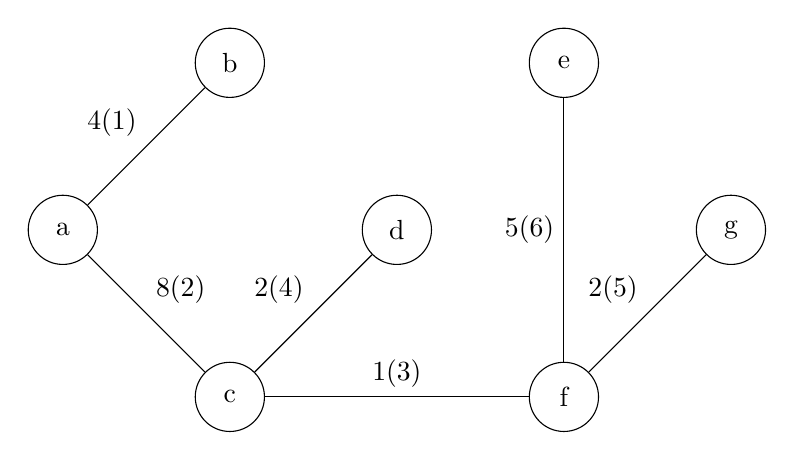
\begin{tikzpicture}[node distance=3cm,bend angle=45,auto]
      \node[state] (n1) {a};
      \node[state] (n2) [above right of = n1] {b};
      \node[state] (n3) [below right of = n1] {c};
      \node[state] (n4) [below right of = n2] {d};
      \node[state] (n5) [above right of = n4] {e};
      \node[state] (n6) [below right of = n4] {f};
      \node[state] (n7) [above right of = n6] {g};

      \path[-] (n1)
        edge node {$4(1)$} (n2)
        edge node {$8(2)$} (n3);

      \path[-] (n3)
        edge node {$2(4)$} (n4)
        edge node {$1(3)$} (n6);

      \path[-] (n6)
        edge node {$2(5)$} (n7)
        edge node {$5(6)$} (n5);
    \end{tikzpicture}
  \end{question}

  \begin{question}
    \centering
    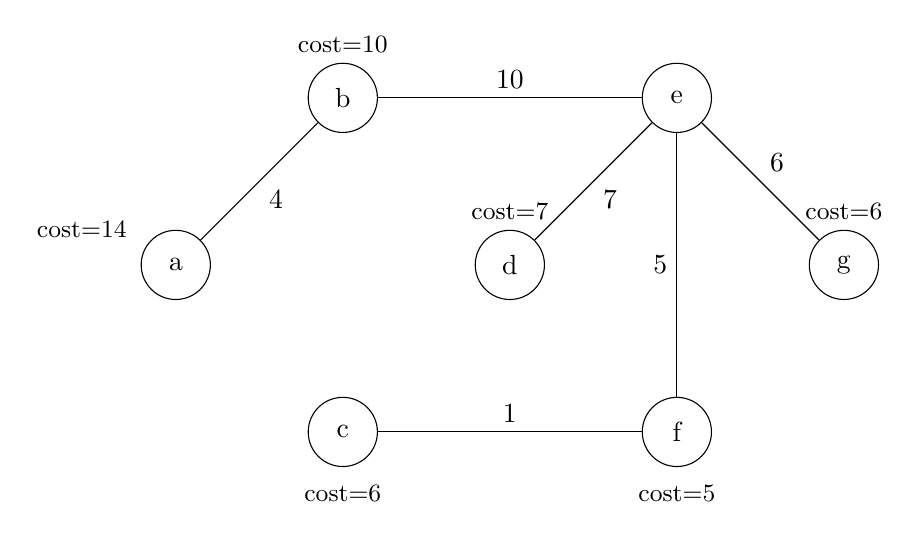
\begin{tikzpicture}[node distance=3cm,bend angle=45,auto]
      \node[state, label={[left = .5cm]\small cost=14}] (n1) {a};
      \node[state, label={[above]\small cost=10}] (n2) [above right of = n1] {b};
      \node[state, label={[below = 1cm]\small cost=6}] (n3) [below right of = n1] {c};
      \node[state, label={[above]\small cost=7}] (n4) [below right of = n2] {d};
      \node[state] (n5) [above right of = n4] {e};
      \node[state,label={[below = 1cm]\small cost=5}] (n6) [below right of = n4] {f};
      \node[state,label={[above]\small cost=6}] (n7) [above right of = n6] {g};

      \path[-] (n3)
        edge node {$1$} (n6);

      \path[-] (n2)
        edge node {$10$} (n5)
        edge node {$4$} (n1);

      \path[-] (n5)
        edge node {$7$} (n4)
        edge node {$6$} (n7);

      \path[-] (n6)
        edge node {$5$} (n5);
    \end{tikzpicture}
  \end{question}

\end{document}
